\documentclass[bsc,frontabs,singlespacing,parskip, twoside]{infthesis}
\usepackage{filecontents}
\usepackage{fancyvrb}
\usepackage{graphicx}
\usepackage[export]{adjustbox}
\usepackage{multirow}

\usepackage{tikz}
\usetikzlibrary{bayesnet}
\usepackage{dirtree}
\usepackage{array}
\usepackage{xcolor, colortbl}
\usepackage{hhline}
\usepackage{chngpage}

\begin{document}
\long\def\/*#1*/{}

\title{Representing Films as Character Graphs}

\author{Victor Dumitrescu}

\course{Artificial Intelligence and Computer Science}
\project{4th Year Project Report}

\date{\today}

\abstract{
This project sets out to explore a representation of films in terms of their characters, bringing together different kinds of textual information, such as screenplays and plot summaries. The work described in this report builds upon the existing literature in computational linguistics concerned with studying characters in films and other works of fiction. The character graphs presented here model two main aspects of film characters: their personalities and their role in the social network of the narrative. We try to show that by using both kinds of features to represent films, we can derive some insight into deeper aspects of the narratives.
}

\maketitle

\section*{Acknowledgements}
Thanks I guess.

\tableofcontents
\listoffigures
\listoftables

\chapter{Introduction}

[\textit{I plan to write this towards the end.}]

\chapter{Context and background}
\label{chap:background}

\section{Background work}
Researchers have been interested in computationally analysing narrative fiction for decades. However, this interest has dramatically increased along with the size of raw data available and the ability to store and process ever-growing data sets. In order to establish the basis of the work described in this report, we will highlight some of the previous literature which takes a character-centric point of view when approaching narrative fiction [TODO also networks, sentiment].

\subsection{The Persona Model}
\label{sec:bg_persona}
Recent work by David Bamman and others has explored the idea of learning the type or \textit{persona} of film \cite{Bamman2013} and literary \cite{Bamman2014} characters. A character persona is a probabilistic model of a character's personality traits, constructed using certain keywords from a film's plot summary. The papers present a number of variations of this model, but we will only describe the \textit{Dirichlet Persona Model} introduced in \cite{Bamman2013}, which serves as the basis for this work.

Instead of trying to build these models of character personality using information conveyed in the films themselves, such as dialogue or descriptions from the screenplays, Bamman and his colleagues relied on summaries of films' storyline, written by human editors on Wikipedia. These are usually concise, straightforward descriptions of the events and characters of a film, written in a neutral style. A more detailed discussion of the this data follows in Section~\ref{sec:data sets}. 

A core assumption in their model is that character personalities are primarily represented by three types of words in the plot summaries:
\begin{itemize}
	\item \textbf{Agent verbs:} Verbs for which the character is an agent (e.g. "Starling \textit{travels} to the victim's hometown")
	\item \textbf{Patient verbs:} Verbs for which the character is the patient or object (e.g. "Starling is \textit{led} to the house of Jack Gordon", where \textit{Starling} is a passive nominal subject)
	\item \textbf{Modifiers:} Other words which describe the characters (e.g. "Catherine is still \textit{alive}")
\end{itemize}
The classification of tokens into one of these categories is based on their Stanford Typed Dependencies \cite{de2008stanford}, assigned using the Stanford CoreNLP natural language analysis toolkit \footnote{http://nlp.stanford.edu/software/corenlp.shtml}.

In their \textit{Dirichlet Persona Model} (Figure~\ref{fig:dirichlet_persona}), these words, along with their classification into the 3 categories described above are the only data used to infer the persona of a character. In addition to this model, they propose an augmented one (\textit{Persona Regression}), which also takes some metadata into account, namely the age and gender of the characters (based on the gender and date of birth of the actor portraying that character) and the genre of the film.

\begin{figure}[ht!]
\centering
\begin{tikzpicture}

  % Define nodes
  \node[obs]                      (w) {$w$};
  \node[latent, above=of w]       (z) {$z$};
  \node[obs, right=of z]          (r) {$r$}; 
  \node[latent, above=of z]       (p) {$p$};
  \node[dash, above=of p]         (theta) {$\theta^{(d)}$};
  \node[latent, left=of theta]    (alpha) {$\alpha$};
  \node[dash, left=of w]          (phi) {$\phi^{(z)}$};
  \node[latent, below=of phi]     (gamma) {$\gamma$};
  \node[dash, left=of z]          (psi) {$\psi^{(r)}$};
  \node[latent, above=of psi]     (nu) {$\nu$};

  \edge {z}{w}
  \edge {r}{z}
  \edge {theta}{p}
  \edge {p}{z}
  \edge {alpha}{theta}
  \edge {phi}{w}
  \edge {gamma}{phi}
  \edge {psi}{z}
  \edge {nu}{psi}

  \plate {zwr} {(z)(w)(r)} {$W$};
  \plate {zwrp} {(zwr)(p)} {$E$};
  \plate {zwrp_theta} {(zwrp)(theta)} {$D$};

\end{tikzpicture}
\caption{Graphical model of the \textit{Dirichlet Persona Model} presented in \cite{Bamman2013}. Figure adapted from the one in the paper. As can be seen when comparing with Figure~\ref{fig:lda} below, it extends the LDA model.}
\label{fig:dirichlet_persona}
\end{figure}

Graphical models are useful for representing dependence relationships between random variables and allowing inference to be modelled in terms of graph operations \cite{barber2012bayesian}. In the notation used in Figure~\ref{fig:dirichlet_persona}, nodes are random variables, directed edges represent dependence and a \textit{plate} (rectangle) shows that a certain random variable is replicated a number of times (shown in the bottom-right corner of the plate). Nodes that are shaded represent observed variables, while dashed nodes signify that they are \textit{soft evidence} for the variable which depends on it, meaning that the probability mass is divided among different states. This is in contrast to \textit{hard evidence}, where all the probability mass rests in one state. Such a relationship defines a \textit{soft-} or \textit{hard-clustering} of the data. In the former case, data points can be assigned to more than one cluster (e.g. words can belong to more than one topic), while in the latter each point is assigned to a single cluster (e.g. characters have a single persona).

In the generative model shown above, the words $w$ and their role $r$ (\textit{agent}, \textit{patient}, \textit{modifier}) are the observed variables. $W$ is the total number of words. Each word is assigned a topic $z$. Topics $\phi$ are multinomial distributions over words in the vocabulary, with a Dirichlet prior, parameterised by $\gamma$. A persona $p$ is then defined as a set of 3 multinomial distributions $\psi$ over the topics, also with a Dirichlet prior, each parameterised by a $\nu_r$. At the document (film) level, characters' personas are also drawn from a multinomial distribution $\theta$, with a Dirichlet prior, parameterised by $\alpha$. The authors use collapsed Gibbs sampling \cite{griffiths2004finding} to sample the latent topic $z$ of each word and the persona $p$ of each character. Performing this type of inference, while optimising all the hyperparameters on a large data set is computationally expensive. This is one of the reasons for which we sought to implement and test a simplified version of this model, described in Section~\ref{sec:persona_impl}, which is based directly on an implementation of Latent Dirichlet Allocation.

\subsection{Social networks in narrative fiction}
Another strand of work in this field is concerned with the interactions between characters and how that contributes to defining the story, rather than with their individual personalities. When analysing narratives and the characters that make up the story, we can think of representations that would capture their interactions and they ways in which they affect the story progression. An intuitive representation is that of a social network: a graph in which nodes are used to denote characters and edges represent some kind of interaction between them. Different variations of this model have been proposed.

Extracting and analysing social networks of characters from works of fiction has already proven valuable for a number of applications. In the context of novels, such an approach can be used to answer literary theory questions by taking into account a large sample of writings, rather then the small subset of well-known works which are usually examined by literary scholars. In their paper \cite{Elson2010}, Elson et al. propose a way in which social networks can be extracted from English novels and set out to answer disputed questions about the correlation between different features of narratives (e.g. first- or third-person perspective, urban or rural setting) and character interactions (e.g. cohesion of the social network). Their approach uses the number and length of quoted speech acts which are inferred to be directed from one character to another to assign a weight to the relationship between the characters.

Others have tried to extend the social network representation beyond quoted speech \cite{Agarwal2013}, also in the context of literary fiction. Using a wider concept of \textit{social events} \cite{agarwal2010annotation}, meant to include any ``deliberate" interaction not captured by direct speech (e.g., using the notation from the paper for characters and social events, ``\{He\} [was looking] at \{Tomas\} and [trying to smile]."\footnote{Kundera, Milan. \textit{The Unbearable Lightness of Being}. Translated by Richmond Hoxie. London: Faber \& Faber, 1984.}), Agarwal et al. proposed a method for automatically extracting social networks from texts and evaluated their result  by comparing their extracted social network from ``The Adventures of Alice in Wonderland" with a gold-standard annotated network, using standard network measures such as degree centrality, betweenness centrality and graph density.

Social network extraction has been attempted in many other contexts, including e-mail conversations, online communities... [TODO]. 

\subsection{Sentiment analysis}
Sentiment analysis is an active area of research which generally aims to reliably detect the subjective feeling or opinion expressed by someone, usually in writing, towards an idea or topic, a product or another person \cite{varghesesurvey}. In the wake of the ``big data revolution" \cite{mayer2013big}, which generated a substantial interest for many organisations to collect and analyse customer data in order to guide their strategies, sentiment analysis (in this context, often called \textit{opinion mining} \cite{pang2008opinion}) became a key technique for gauging the interest and reactions of the public automatically, on an unprecedented scale. One of the most common sentiment analysis tasks, especially important for industrial applications, is detecting \textit{sentiment polarity}: deciding whether the sentiment expressed (e.g. in a product review, a tweet, a blog post) is positive or negative.

Success in any sentiment analysis tasks is subject to overcoming many challenges, some of them related to limitations in state-of-the-art natural language processing tools in general, but others specific to the domain. One major obstacle, which seems to be inherent to dealing with subjectivity, is the fact that the accuracy of any such system is limited by the rate of agreement between human judgements. Different studies found that humans will agree on the sentiment polarity of a sentence between 75\% and 90\% of the time \cite{godbole2007large, wilson2005recognizing}. Another difficulty in building automatic sentiment analysis systems is that the way in which people express feelings can be different depending on the context (e.g. product reviews and film reviews) \cite{varghesesurvey}, meaning that systems which perform well in one domain will not necessarily generalise. Sentiment analysis also depends on reliably performing generic NLP tasks, such as named entity recognition, co-reference resolution and dependency parsing\footnote{These concepts will be explained in Section~[TODO ref], when discussing the implementation of the text processing pipeline for the project.}, which are still not completely solved problems.

\subsubsection{Approaches to automatic sentiment analysis}

There are a number of general-purpose and domain-specific sentiment analysis systems in wide use today.

Sentiment analysis is usually broken down into different levels of granularity and treated differently in each case \cite{liu2012sentiment}:
\begin{itemize}
	\item \textbf{Phrase level}
	\item \textbf{Sentence level} 
	\item \textbf{Document level} Assessing the sentiment of a document as a whole (i.e. a text composed of multiple sentences, such as a blog post) assumes that it expresses a single, coherent point of view about a single topic. Therefore, it has limited applicability, since this assumption often does not hold in practice.
\end{itemize}

\subsubsection{The VADER sentiment analysis system}

For this project, we used VADER (\textit{Valence Aware Dictionary for sEntiment Reasoning})\cite{hutto2014vader}, a rule-based sentiment analysis system, geared towards analysing social media content. It is implemented in Python and it is available as an open-source project under the MIT licence\footnote{https://pypi.python.org/pypi/vaderSentiment}.


\subsection{Sentiment analysis in the study of fiction}
First work in sentiment analysis on works of fiction \cite{alm2005emotions}, on children's fairy tales.

Alm et al. also explore the role of ``emotion trajectories" in story development. \cite{alm2005emotional}.

Building on this previous work and on that of Elson et al., Elsner uses sentiment trajectories of individual characters rather than entire narratives \cite{elsner2012character}.

All these previous works focus on literary fiction rather than films.

Sentiment analysis and social networks. (Philip Gorinski used it in summarisation)

The main basis for the sentiment work in this project: \cite{Nalisnick2013} sentiment trajectories of individual characters based on speech acts in plays, adapted for films.

\section{Data sets} \label{sec:data sets}
We have mainly used two data sets to support the work done for this project. They have both been compiled as part of previous research efforts focused on computationally analysing films.

\subsection{The CMU Movie Summary Corpus}
A collection of 42,306 Wikipedia plot summaries of films, along with metadata extracted from Freebase. The summaries are processed using the \textit{Stanford CoreNLP} tools, specifically tagging, parsing, named entity recognition and coreference resolution.

\subsection{ScriptBase}
ScriptBase \cite{Gorinski2015} is a corpus of 1,276 film scripts, along with IMDB and Wikipedia metadata. Of these, 127 have been similarly processed using the \textit{Stanford CoreNLP} pipeline and standardized as XML files following a set schema.

[TO DO: \textit{More details on what kind of data is extracted in these corpora and specific pre-processing steps}]

[Wiki on plot summaries: "The plot summary is an overview of the film's main events, so avoid minutiae like dialogue, scene-by-scene breakdowns, individual jokes, and technical detail."]

\chapter{Aims and hypotheses}
\label{chap:aims}

The aims of this project were to explore different representation of films and identify what kinds of features can be captured by these representations. A big part of the work done as part of the project was directed at probing these possibilities, by constructing variations of the character graph representation and measuring their effectiveness using a number of prediction tasks. Inevitably, not all of them produced significant results or were even practical to test. Along with our main hypothesis, we will present some of the work which did not yield any fruit and discuss the underlying reasons.

\section{Inter-character sentiment}
In one sentence, the main hypothesis is that character graph representations can be used to predict inter-character sentiment. As discussed in Chapter~\ref{chap:background}, there have been previous attempts to link character social networks and some form of sentiment analysis. By using character personas and a measure of the strength of two characters' relationships to predict aspects of the sentiment in speech acts directed from one character to the other, we can bring together two distinct aspects of film narratives and show that they correlate. On the level of the text resources used, we link the raw dialogue of a film (from the film scripts) and the human-produced plot summaries. On the narrative level, we correlate the \textit{actions} of characters (as described in the plot summaries) with their utterances. [\textit{Note: I think this is really interesting, but I'm not sure how to develop it.}]

\section{Alternative hypotheses}

This section presents two of the hypotheses which were strongly considered and explored and discusses why they were not feasible to test. More details on the design and implementation of the code written to investigate them are included in the next chapter (Section~\ref{sec:alt_hyp_implementation}).

\subsection{TV Tropes}
TV Tropes\footnote{http://tvtropes.org/} is an online public wiki maintaining a collection of ``tropes", such as plot devices, dialogue commonalities, motifs and other conventions or stereotypes that are widely used in film and television series. More recently it ha also grown to include literature, video games and other media. Apart from collecting the tropes themselves, TV Tropes maintains pages for numerous individual films and other works of fiction which include a list of the tropes that they feature.

TV Tropes have been used in past research efforts, most notably by Bamman et al. \cite{Bamman2013}, as part of one of the evaluation measures for their film persona models introduced in Section~\ref{sec:bg_persona}. They selected 72 tropes which correspond to character types (e.g. \textit{The Hardboiled Detective}) and manually annotated 501 characters. They attempted to recover gold-standard clusters of characters as determined by their trope assignment and used an information-theoretic measure to assess the discrepancy between these and the latent persona clusters.

We considered the possibility of evaluating our character graph representations on the basis of being able to capture different kinds of relationships between 2 or more characters (e.g. one of the \textit{Triang Relations}\footnote{http://tvtropes.org/pmwiki/pmwiki.php/Main/TriangRelations} or \textit{Four-Man Band}. For this purpose, we have implemented a scraper in order to collect the tropes associated with the films in our data set. Table~\ref{table:tropes} shows the most common 20 tropes and the number of films which feature them.

\newcolumntype{L}[1]{>{\raggedright\let\newline\\\arraybackslash\hspace{0pt}}m{#1}}
\begin{table}[h!]
\centering
\begin{tabular}{|c||L{4.5cm}|l|c|c||L{4.5cm}|l|}
\cline{1-3} \cline{5-7}
1 & Shout-Out & 54 & & 11 & Berserk Button & 22 \\ \cline{1-3} \cline{5-7}
2 & Deadpan Snarker & 31 & & 12 & Cluster F-Bomb & 19 \\ \cline{1-3} \cline{5-7}
3 & Lampshade Hanging & 27 & & 13 & Butt Monkey & 18 \\ \cline{1-3} \cline{5-7}
4 & Chekhov's Gun & 27 & & 14 & Large Ham & 18 \\ \cline{1-3} \cline{5-7}
5 & Running Gag & 26 & & 15 & Badass & 18 \\ \cline{1-3} \cline{5-7}
6 & Oh, Crap & 25 & & 16 & Ax-Crazy & 18 \\ \cline{1-3} \cline{5-7}
7 & Brick Joke & 24 & & 17 & Title Drop & 17 \\ \cline{1-3} \cline{5-7}
8 & Precision F-Strike & 23 & & 18 & Word Of God & 17 \\ \cline{1-3} \cline{5-7}
9 & Foreshadowing & 23 & & 19 & Meaningful Name & 16 \\ \cline{1-3} \cline{5-7}
10 & Black Comedy & 22 & & 20 & Even Evil Has Standards & 16 \\ \cline{1-3} \cline{5-7}
\end{tabular}
\caption{The 20 most frequent TV Tropes and the number of films which feature them (out of the 83 films in the collection)}
\label{table:tropes}
\end{table}

None of these 20 tropes describe character relationships in any way. Most of them capture plot devices, features of speech or stylistic choices. Lacking a significant number of films (all other tropes are featured in less than 16 films) which include any kind of stereotypical and easily identifiable character relationships, we were not able to use TV Tropes to evaluate the character graph representation.

\subsection{Film similarity}
\label{sec:hyp_film_sim}
Another evaluation measure considered for assessing the usefulness of character graphs was the ability to compare them in order to predict film similarity, as judged by human raters. In principle, we would expect to obtain at least some degree of accuracy, although film similarity can depend on contextual information beyond the dialogue or narrative of a film. Of course, most recommender systems determine film similarity based on users' reviews and activity and on metadata (e.g. genre, year, cast, crew) rather than the content of the films themselves \cite{said2010putting}.

Some of the reasons for which we were not able to test this hypothesis are the small size of our film corpus and the fact that the films were quite diverse, resulting in very few similarity relations between them. Furthermore, graph comparison is a difficult problem, highly specific to the domain. There are no universal solutions, but some work has been made on comparing graphs of social networks \cite{macindoe2010graph}. A fuller discussion of our attempts to investigate this hypothesis follows in the chapter on Design and Implementation (Section~\ref{sec:test_film_sim}). This is because it relies on details and explanations given in subsequent sections.

\chapter{Design and Implementation}

This chapter details the components of the software pipeline implemented as part of the project to acquire and process data, construct character graphs and carry out experiments. The system was primarily programmed using Python 2.7.6. The language was chosen for the terse and flexible style of programming that it enables and for its adoption in the NLP community, having a large ecosystem of libraries and tools developed around it. Some parts concerned with parsing script files and gathering film similarity judgements from Rotten Tomatoes were implemented using F\# 3.1. This choice was made on the basis of F\#'s smooth integration with external data sources and ease of working with schematised data.

The structure of the Python project is shown in Figure~\ref{fig:dirtree}. Directories and source files in the root directory correspond to the major areas of implementation, which can roughly be categorised as follows (by directory/file):
\begin{itemize}
	\item \texttt{\textbf{topics}}:  Extract and filter plot summary data, run Latent Dirichlet Allocation and pickle the resulting topic distributions
	\item \texttt{personas.py}: Define a \texttt{Persona} class, compute the persona for each character and pickle them
	\item \texttt{graphs.py}: Construct character graphs and implement various functions for working with them (e.g. filter nodes/edges)
	\item \texttt{film.py}: Define a \texttt{Film} class, which stores the character graphs and matches them with various pieces of metadata (e.g. title, year, names of characters)
	\item \texttt{\textbf{sentiment}}: Extract speech acts from processing film scripts and construct sentiment trajectories between pairs of characters
	\item \texttt{\textbf{prediction}}: Implements various predictors and tools for feature engineering and running repeated experiments with different configurations
	\item \texttt{\textbf{utils}}: Processing raw data, pickling and other utility functions required throughout the project
\end{itemize}

The names of the rest of the source files give a good indication of what functionality they implement and should serve as a guide for exploring the source code.

\hspace{.1in}
\begin{figure}[ht!]
\dirtree{%
.1 \textbf{python}.
.2 \textbf{topics}.
.3 acquire\_vocab.py.
.3 filter\_genres.py.
.3 model\_topics.py.
.2 \textbf{sentiment}.
.3 trajectories.py.
.2 \textbf{prediction}.
.3 decision\_tree.py.
.3 random\_forest.py.
.3 svm.py.
.3 lin\_regression.py.
.3 ridge\_regression.py.
.3 regression\_tree.py.
.3 svm\_regression.py.
.3 features.py.
.3 predict.py.
.2 \textbf{utils}.
.3 filter\_summaries.py.
.3 process\_summaries.py.
.3 process\_scripts.py.
.3 store\_sentiment.py.
.3 misc.py.
.2 films.py.
.2 personas.py.
.2 graphs.py.
.2 compare.py.
.2 run\_topic\_model.py.
}
\caption{General structure of the Python code written for the project}
\label{fig:dirtree}
\end{figure}

The code for constructing the Rotten Tomatoes film similarity graph was written in F\#. Its structure is outlined in Figure~\ref{fig:fsharpdirtree}.

\begin{figure}[th!]
\dirtree{%
.1 \textbf{\texttt{rtgraph}}.
.2 Graph.fs.
.2 ApiCalls.fs.
.2 ToGEXF.fs.
.2 Main.fs.
}
\caption{General structure of the F\# code written for the project}
\label{fig:fsharpdirtree}
\end{figure}

\section{The Character Graph}
In order to construct the character graph for a film we need to find a meaningful representation of the relationship between characters (the nodes in our graph). For simplicity, we can start by trying to find a numerical measure, which would correspond to edge weights in an undirected weighted graph. The measure we have used in this project is the number of scene co-occurrences between two characters. Thus, the weight of an edge between two characters represents the number of scenes in which those characters appear together. As a consequence, characters which never interact in the film will be disconnected in the graph. 

Apart from simplicity, choosing this measure can enable us to reliably discover the main characters of a film using a graph centrality indicator. However, scene co-occurrence does not give any insights into the \textit{nature} of the interaction between characters, but a high co-occurrence is likely to indicate that a relationship is important for the development of the story.

\subsection{Processing ScriptBase screenplays}
\label{sec:processing_scriptbase}
To ease the task of extracting the number of character to character scene co-occurrences, we restricted the set of films to the 127 which have already been processed in ScriptBase. A processed script is an XML file which, apart from the standard CoreNLP annotations, also places every sentence inside a numbered \texttt{scene} tag. It also distinguishes between stage directions and speech, annotating the name of the speaker(s) in the latter case.

Thus, it is straightforward to parse the XML document and, for each pair of characters, record the number of scenes in which they both have at least one line of speech. Note that although this approach ignores characters which might be present in a scene but do not speak, in practice we do not expect this to significantly influence any of the results.

\subsection{Constructing character graphs}
For generating and storing character graphs, we have chosen the GEXF format\footnote{The GEXF file format, \textit{www.gexf.net}}, a standard XML format for describing general network structures. As described above, we extract all the character names from the script and use them as the set of nodes in the graph. We add a weighted edge for all the recorded interactions between characters. As a result, each of the 127 films in the data set will be represented with a GEXF file.

\begin{figure}
	\centering
	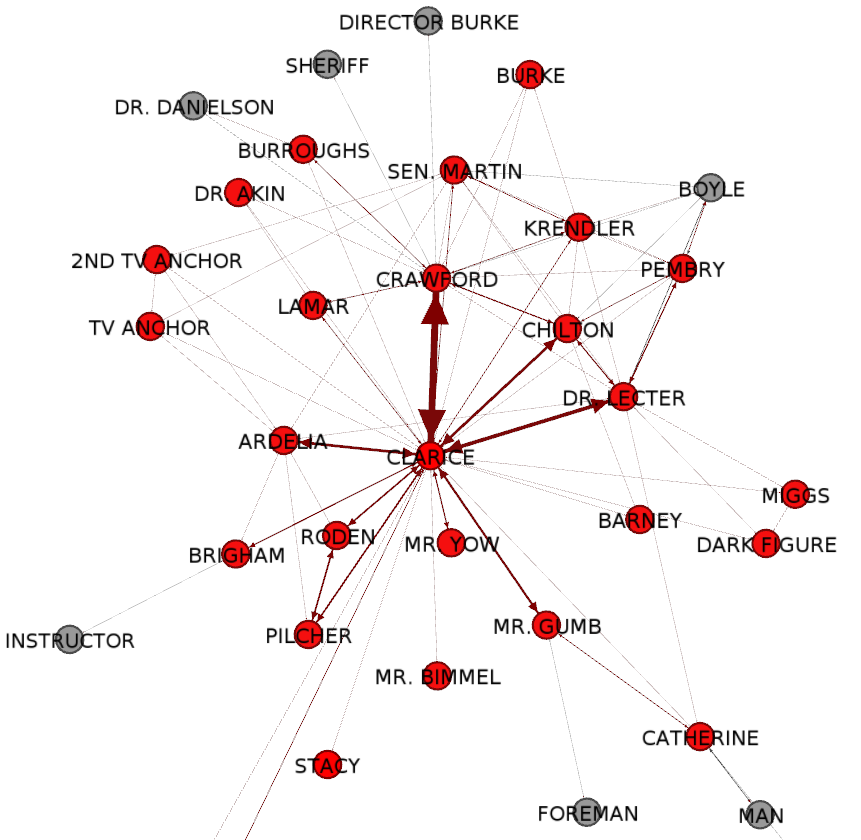
\includegraphics[scale=0.4]{figures/clarice_graph}
	\caption{The character graph of \textit{The Silence of the Lambs} (1991), centred around the protagonist, Clarice Starling. Red vertices are those adjacent to Clarice (characters with which she interacts). Edge width is proportional to the number of scene co-occurrences between two characters.}
\end{figure}

Once the character graphs are constructed, the nodes can be annotated with the persona information. Note that although the character graphs are likely to contain a node for every character in the plot (a small variation can occur due to faults in the preprocessing of scripts), personas will be computed for 2-5 main characters. Again, due to the limitations of the standard NLP tools (most notably coreference resolution), this number can be lower, sometimes even 0. To work with annotated graphs in our project, we have used the Python \texttt{networkx} library \footnote{www.networkx.github.io}, which can be used for complex graph modelling and implements many useful graph algorithms and network measures.


\section{The Persona Model}
\label{sec:persona_impl}
We implemented a simplified version of the Dirichlet Persona Model introduced by Bamman et al. \cite{Bamman2013} and described in Section~\ref{sec:bg_persona}. 

\subsection{Processing the CMU script summaries}
\label{sec:processing_cmu}
The CMU corpus provides both the raw plot summaries and a file containing all the processed summaries, which can be used as input for the pipeline described in their paper. We have designed ours to work with the same input format, enabling us to use the data from this corpus without any additional preprocessing, apart from filtering out the films for which we have not constructed a character graph. This includes the majority of films in the corpus. Out of the 127 films from ScriptBase, 96 also have a processed plot summary. This films in this intersection are the starting point in our processing pipeline.

\begin{figure}[h]
\centering
\begin{minipage}{14.5cm}
\begin{Verbatim}[frame=single]
30006 /m/0k6g8c:t0.1.0:verb.contact:pull:a:agent /m/0k6g8p:t2.2.0
:verb.stative:lead:a:agent /m/0k6g86:t3.0.0:verb.change:grow:a:ns
ubj /m/0k6g86:t3.2.0:verb.communication:rebuff:a:nsubj (...)
\end{Verbatim}
\end{minipage}
\caption{A an entry (corresponding to a film) in the input file used for the work described in \cite{Bamman2013}, which we filtered and used as input for this project.}
\label{fig:bamman_input}
\end{figure}


The filtered film data file contains, for each film and each character mentioned in the plot summary, a list of words tagged as being either \textit{agent}, \textit{patient} or \textit{modifier} words (as detailed in Section~\ref{sec:bg_persona}). These words are selected into one of these types on the basis of their Stanford typed dependencies, as determined using the CoreNLP parser. Each of the three types described above corresponds to a list of dependencies and all tokens tagged with those dependencies will be assigned a type. In the final input file, in addition to the word lemma, its type (agent, patient, modifier) and its dependency tag, the word tuples for each character also contain the part of speech and the WordNet supersense. As show in Figure~\ref{fig:bamman_input}, each line starts with the identifier of the film, followed by a list of (colon-separated) tuples, containing this data. The first item in the tuple will either be a Freebase\footnote{Freebase (www.freebase.com) is a Google-owned, community-driven repository of structured data, containing numerous topics, entities and connections between them. Each entity has a unique ID.} identifier or have the format \texttt{eXX} (where \texttt{XX} stands for a 2 digit number) for characters and other entities which could not be matched with Freebase entities. The full preprocessing pipeline, with a sample sentence as a running example is outlined in Appendix~\ref{appendix:cmu}. Note that Bamman et al. provide both the data and the code required to produce it\footnote{www.ark.cs.cmu.edu/personas/}.


\subsection{Constructing the persona model}
In this project we implement a simplified version of the Dirichlet Persona Model. The original model was implemented as generative model. In the paper, a persona is defined as a set of 3 distributions (corresponding to agent, patient and modifier words) over topics, which are in turn distributions over words, similar to topic in Latent Dirichlet Allocation.

We have opted to use an implementation of the standard Latent Dirichlet Allocation \cite{Blei2003} algorithm, using the \texttt{lda 0.3.2} Python package \footnote{ www.pypi.python.org/pypi/lda} in order to derive the latent topics in our vocabulary and use a simple maximum likelihood estimation method to compute each character's 3 distributions over these latent topics.

\begin{figure}[h!]
\centering
\begin{tikzpicture}

  \node[obs]                               (w) {$w$};
  \node[latent, above=of w]                (z) {$z$};
  \node[dash, above=of z]              (theta) {$\theta^{(d)}$};
  \node[latent, left=of theta]        (alpha) {$\alpha$};
  \node[dash, left=of w]                 (phi) {$\phi^{(z)}$};
  \node[latent, below=of phi]          (gamma) {$\gamma$};

  \edge {z}{w}
  \edge {theta}{z}
  \edge {alpha}{theta}
  \edge {phi}{w}
  \edge {gamma}{phi}

  \plate {zw} {(z)(w)} {$W$};
  \plate {zwt} {(zw)(theta)} {$D$};

\end{tikzpicture}
\caption{Graphical model for Latent Dirichlet Allocation (LDA)}
\label{fig:lda}
\end{figure}

One of the advantages of this frequentist approach is that the only parameter that we need to optimise in the model is the number of topics computed by the LDA algorithm. Since the number of films in our collection is small and largely restricted to two genres (thriller and comedy), we expect the number of meaningful topics to also be reasonably small. Therefore we have tried to manually vary this parameter and select the value which seems to intuitively give a complete coverage of topics, without having different topics which seem very close. We have used to highest probability words in each topic distribution as a guide. So far, we have settled on having 10 topics (\textit{Figure 1.2}).

\begin{figure}[h]
\begin{minipage}{14.6cm}
\begin{Verbatim}[frame=single]
1: leave meet reveal wife marry ask decide call woman want husband
2: father mother child son marry parent live brother daughter woman
3: kill shoot take man officer arrest escape kidnap detective lead
4: kill rescue escape save arrive bring reveal destroy vampire fly
5: tell be ask see say call friend talk show start mother invite
6: run get chase catch throw grab pull knock hit fall stop walk use
7: friend girl meet student play teacher end girlfriend school 
8: find take follow driver travel hoin reach fly track locate sail
9: kill man shoot attack killer stab die dead confront attempt
10: boy win play have owner manager hero uncle narrator stooge
\end{Verbatim}
\end{minipage}
\caption{Most representative word for each of the 10 topics learned by LDA on all the comedies and thrillers in the CMU Movie Summary Corpus, ranked by probability.}
\label{topics}
\end{figure}

Having these 10 distributions over words in the vocabulary, we construct, for each character, a set of 3 distributions over these topics, by multiplying the number of different occurrences of a certain word lemma with the probability of that lemma in a certain topic, then normalising. It is then easy to compare the persona of two different characters, by using any distance measure, such as Euclidean distance.


\section{Sentiment trajectories}
The sentiment trajectory of a film is the ordered sequence of speech acts, in which one (and only one) character (\textit{the speaker}) is assumed to speak to one (and only one) other character (\textit{the receiver}), which is different than the speaker. The sentiment of each line of dialogue is independently computed, using VADER. Each point in the sentiment trajectory is then a tuple of \textit{(speaker, receiver, sentiment)}, which we will call a \textit{sentiment event}.

In order to construct a sentiment trajectory for each film in the data set, we traverse the XML script (described in Section~\ref{sec:processing_scriptbase}), extract every scene and the names of the characters which take part and every line of dialogue, together with its speaker. The speaker of each utterance is marked in the script, but we nee to identify a receiver. We will follow the assumptions introduced in \cite{Nalisnick2013}:
\begin{itemize}
	\item For the first line of dialogue in the scene, assume the receiver is the next speaker.
	\item For all the following lines, assume the receiver is the previous speaker.
\end{itemize}

Although these assumptions (and those introduced in the first paragraph, restricting dialogue between exactly two distinct characters) are quite “na\"{\i}ve, in practice they tend to hold reasonably well, especially since many scenes only feature 2 participants.

Another assumptions that we make when using the sentiment trajectories as representations of two characters' relation is that the sentiment expressed in a speaker's utterance is directed towards the receiver. Of course, this might not always be the case. To remedy this, we could attempt to parse the typed dependencies from each sentence and only use the phrase-level sentiment from phrases which have a relevant dependency relations with the receiver (e.g. \textit{nsubj}, \textit{dobj}, \textit{ref}, ...), coupled with coreference resolution to match characters with identifier such as ``you", ``your", etc. However, this approach could result in far sparser sentiment trajectories. In practice, although a line of dialogue might not be directly referring to the other party, its sentiment can often be taken as an indicator of the speaker's relationship with the receiver. To minimise the impact of outliers resulting from either a failure of the sentiment analysis or the breaking of one of the assumptions introduced above, we will only use aggregate measures of the sentiment trajectory in our evaluation tasks, discussed in Chapter~\ref{chap:results}.

Once constructed, sentiment trajectories can be plotted as a time series. For clarity, we will only include one character relationship per plot. Note, however, that relationships are directional, since the sentiment that each character expresses towards the other will differ. The plots shown here are illustrative of certain aspects related to the genre or the dynamic between the characters shown. 

\begin{figure}[h!]
\begin{adjustwidth}{-0.5in}{-0.5in}
	\centering
	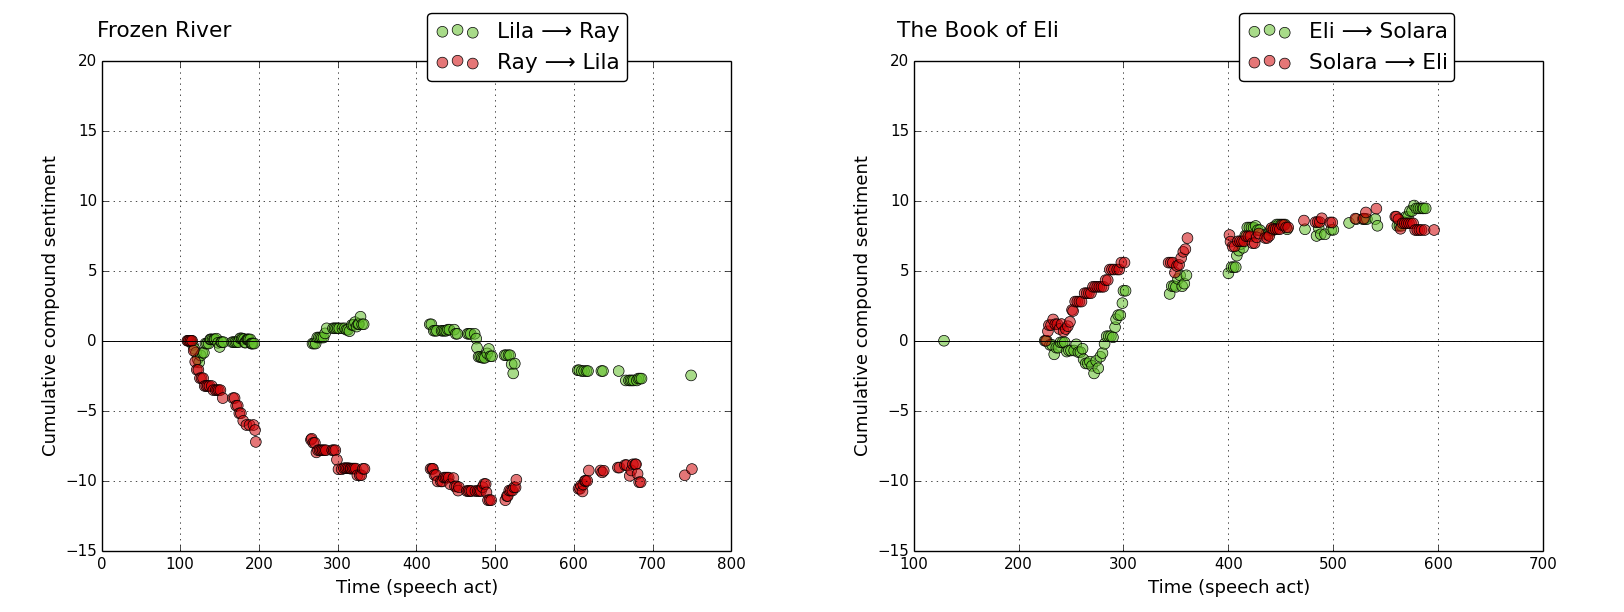
\includegraphics[scale=0.43]{figures/y_thrillers}
	\caption{Sentiment trajectories of the two most central characters in the thrillers \textit{Frozen River} (2008) and \textit{The Book of Eli} (2010)}
	\label{fig:thrillers}
\end{adjustwidth}
\end{figure}

\begin{figure}[h!]
\begin{adjustwidth}{-0.5in}{-0.5in}
	\centering
	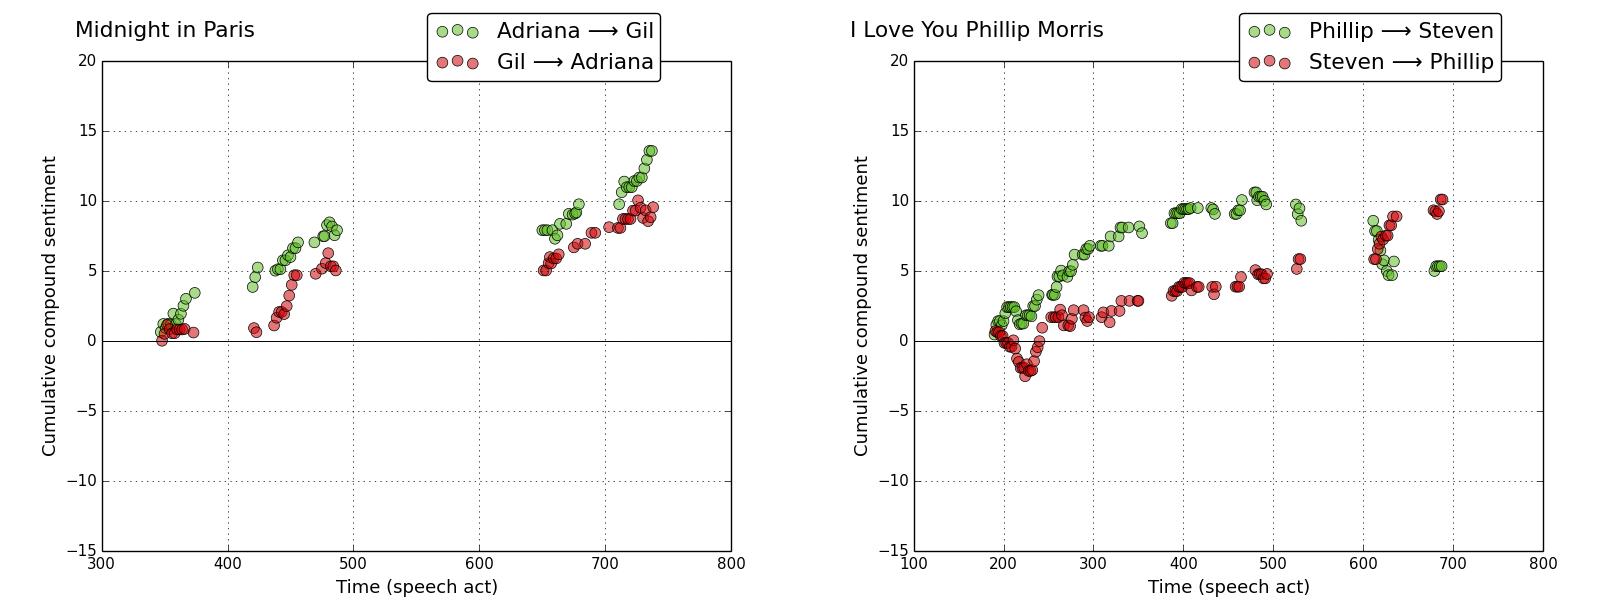
\includegraphics[scale=0.43]{figures/y_romcoms}
	\caption{Sentiment trajectories of the two most central characters in the romantic comedies \textit{Midnight in Paris} (2011) and \textit{I Love You Phillip Morris} (2009)}
	\label{fig:romcoms}
\end{adjustwidth}
\end{figure}

Figure~\ref{fig:thrillers} shows the sentiment trajectories of two thrillers. Both the main characters are allies in the story, but the protagonists of \textit{Frozen River} have a very uneasy alliance, while those in \textit{The Book of Eli} are sympathetic towards each other.

\begin{figure}[h!]
\begin{adjustwidth}{-0.5in}{-0.5in}
	\centering
	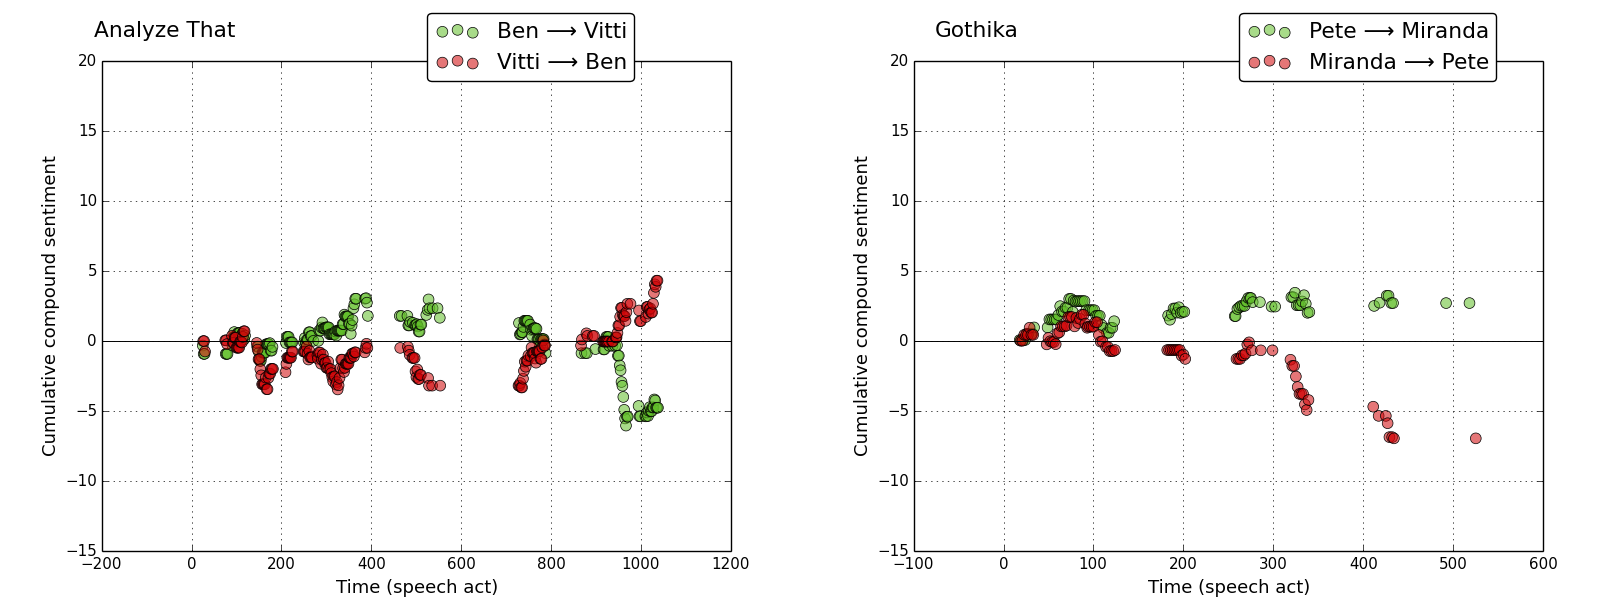
\includegraphics[scale=0.43]{figures/y_contradictions}
	\caption{Sentiment trajectories of the two most central characters in the films \textit{Analyze That} (2002) and \textit{Gothika} (2003)}
	\label{fig:contradictions}
	\label{fig:romcoms}
\end{adjustwidth}
\end{figure}

The sentiment trajectories in Figure~\ref{fig:chasing_amy}[TODO] illustrate the sentiment between the main characters of the romantic comedy \textit{Chasing Amy}. In the film, Holden and Banky are two long-time friends. When the two meet Alyssa, she immediately piques Holden's interest. Although she only sees him as a friend, he pursues her throughout the film and they end up being together. Banky does not like Alyssa, which is the source of conflict between him and Holden. The 3 sentiment trajectories are consistent with our intuitive expectations of such a story and the feelings that the characters would express towards each other in these situations.
\begin{figure}[h!]
\begin{adjustwidth}{-0.5in}{-0.5in}
	\centering
	\begin{minipage}{15cm}
		\centering
		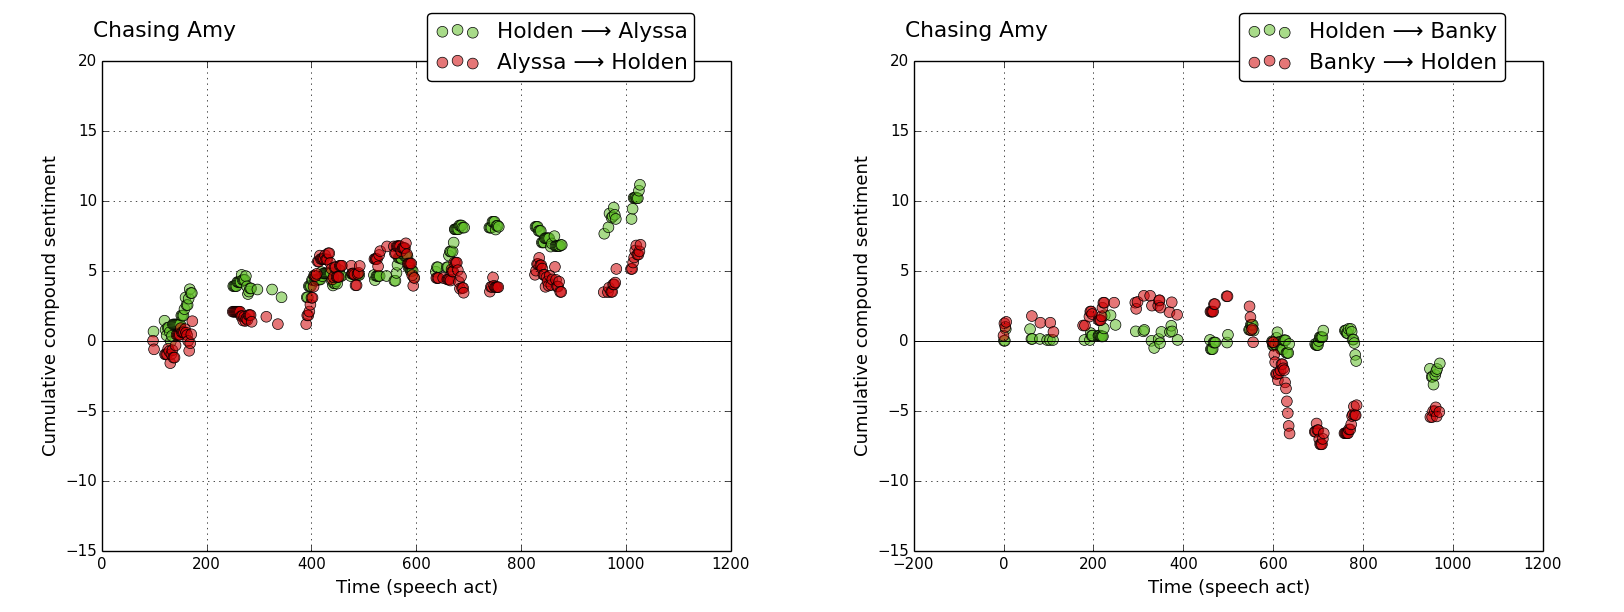
\includegraphics[scale=0.43]{figures/chasing_amy1}
		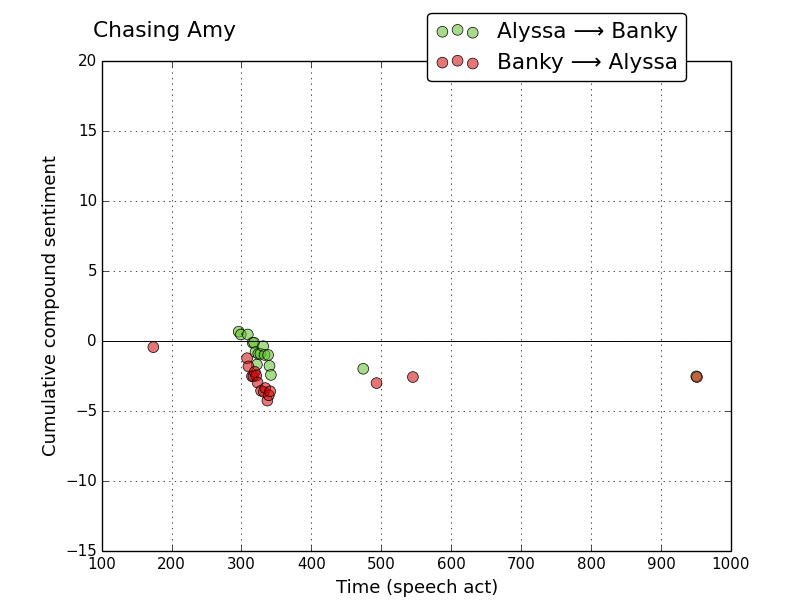
\includegraphics[scale=0.43]{figures/chasing_amy2}
	\caption{Sentiment trajectories of the three most central characters in the romantic comedy 
\textit{Chasing Amy} (1997)}
	\end{minipage}
\end{adjustwidth}
\label{fig:chasing_amy}
\end{figure}


\section{Testing the main hypothesis}
\label{sec:predictors}
In order to test the main hypothesis, a number of prediction tasks were considered, including both classification and regression problems. The tasks themselves and the results are detailed more fully in Chapter~\ref{chap:results}. Here, we will outline the main machine learning techniques used, the reasons for choosing them and their implementation. The toolkit used for carrying out machine learning tasks was the \textit{scikit-learn}\footnote{http://scikit-learn.org/stable/} Python library. It was used for the implementation of the predictors described below, for evaluating the trained models using cross-validation and for generating confusion matrices.

\subsection{Classification}
[TODO: Define each of these predictors]
\begin{itemize}
	\item \textbf{Decision trees:} Used the \texttt{DecisionTreeClassifier} class implemented in \textit{scikit-learn}.
	\item \textbf{Random forests}
	\item \textbf{Support vector machines}
\end{itemize}


\subsection{Regression}
[TODO: Define each of these predictors]
\begin{itemize}
	\item \textbf{Linear regression}
	\item \textbf{Ridge regression}
	\item \textbf{Decision tree regression}
	\item \textbf{SVM regression}
\end{itemize}

\section{Testing the alternative hypotheses}
\label{sec:alt_hyp_implementation}

\subsection{Scraping the TV Tropes website}
[TO DO: \textit{Outline implementation of scraper}]

\subsection{Comparing character graphs}
\label{sec:test_film_sim}

\subsubsection{Direct matching based on centrality}
As discussed in Section~\ref{sec:hyp_film_sim}, graph comparison is a difficult problem which requires careful consideration of the domain. When exploring the film similarity hypothesis, we implemented a simple comparison measure that is based on matching characters from different graphs by their role in the social network. Using degree centrality, the nodes of each graph are sorted and only the first 10 nodes are kept. This parameter can in principle be experimentally adjusted, but we have set it to 10 because for every film in the collection, we could not compute a persona for any character that has rank below 10 by degree centrality. This is not surprising, since plot summaries will rarely mention characters of low importance (assuming importance in the social network translates as importance to the narrative).

Then, every pair of corresponding characters (by rank) in the two graphs is compared. Note that although a persona is a set of 3 distributions, not all characters will have a distribution defined for all 3 types (agent, patient, modifier), since the relevant word lemmas might not be present in the plot summary. Therefore, we compare the distributions which both characters have in common, by taking the norm of the difference between the 2 vectors. The film similarity score is computed as the average of these differences: the lower the score, the more similar the graphs are deemed to be.

\begin{figure}[h]
\centering
\begin{minipage}{11.5cm}
\begin{Verbatim}[frame=single]
Star Trek V    - The Anniversary Party     (0.00167)
Ghost World    - I Love You Phillip Morris (0.00193)
Ghost World    - Copycat                   (0.00202)
Ghost World    - Clerks                    (0.00236)
Ghost World    - Miller's Crossing         (0.00257)
Ghost World    - Nick of Time              (0.00275)
Ghost World    - Sweeney Todd              (0.00338)
The Informant! - The Hangover              (0.00351)
Ghost World    - Gothika                   (0.00352)
Jaws           - Living in Oblivion        (0.00410)
\end{Verbatim}
\end{minipage}
\caption{The 10 most similar pair of films in our collection of 96 thrillers and comedies, based on comparing personas matched by degree centrality rank}
\end{figure}

In these results, it is easy to see that the comedy \textit{Ghost World} (2001) dominates the similarity pairings, being matched both with comedies and thrillers. Overall, the results do not seem to be very revealing. To understand why this might be the case, let us explore the example of \textit{Ghost World}, by showing the top 10 characters and the top 3 topics for each character that has a persona defined. Each topic is described by the top 3 most probable words in that topic.

\begin{figure}[h]
\centering
\begin{minipage}{9cm}
\begin{Verbatim}[frame=single]
ENID 
REBECCA [ M(join wife know)
          M(pursue criminal escape)
          M(girl son offer) ]
SEYMOUR [ P(tell take go)
          A(tell take go)
          A(meet discover leave) ]
ROBERTA [ A(give kill confront)
          A(girl son offer)
          M(girl son offer) ]
JOE 
CUSTOMER 
PAUL 
GERROLD 
JEROME 
STEVEN 
\end{Verbatim}

\end{minipage}
\caption{The 10 most central characters in \textit{Ghost World} and their personas}
\end{figure}

One explanation for the dominance of \textit{Ghost World} in the similarity results shown above is the fact that its characters seem to be typical of both romantic comedies (topics such as \texttt{(join wife know)} or \texttt{(meet discover leave)}) and thrillers (topics like \texttt{(give kill confront)}).

We suspect that one of the causes of the weak results is the small number of films in our collection and, consequently, the small number of words in the vocabulary. This can lead to a topic clustering which does not have much discriminative power (see the list of topics in Figure \ref{topics}). It might also be the case that, since not many personas are matched between films, these occasional matches might be insufficient for obtaining meaningful results across the whole corpus.

\subsection{Rotten Tomatoes similarity}
In order to test the film similarity hypothesis, independent of the work described so far, we have also tried to construct a gold-standard collection of film similarity pairs, using data supplied by Rotten Tomatoes\footnote{www.rottentomatoes.com}. Their public API supports requests of the form "What films have users deemed to be similar to this one?" and offers up to 5 results.

We have found that the results obtained by querying every film in the collection and discarding every returned film which is not part of the collection yields a very small number of pairs. Thus, we have expanded the similarity measure by constructing a graph in which films are nodes and edges represent similarity and allowing films from outside the corpus. The similarity can then be measured as the minimum distance in the graph.

However, the limited number of films in our collection and the fact that they are quite diverse (i.e. it is difficult to find pairs for which human judgements indicate similarity) meant that we could not meaningfully assess whether character graphs can be used to predict general film similarity. 

\chapter{Results and discussion}
\label{chap:results}

From its onset, this project was exploratory in nature. Experimenting with various film representations and the kinds of features that they can reliably predict was one of the main goals. As detailed in Chapter~\ref{chap:aims}, the main hypothesis we chose to explore is whether the character graph representation of films can be used to predict inter-character sentiment. The results presented in this chapter and the subsequent discussion will offer some insight into how this can be achieved. We will examine different ways in which persona information and character relationships can be combined. We ran a large number of experiments, exploring different transformations of the feature space and various machine learning techniques. This chapter will provide an overview of the types of prediction problems attempted, report interesting experimental results and attempt to discuss their significance.

\section{Experimental setup and data transformations}
The same experimental setup and basic data is used for all of the prediction tasks detailed below. The starting point is the set of 876 character-to-character relationships, described by the persona of each character and the weight of the edge between the nodes in the character graph. Since our topic model has 10 topics and each persona is a set of 3 distributions over the latent topics, each feature vector will have size 61 ($2 \cdot 30$ persona variables $+ 1$ edge weight). Each feature vector will have an associated label, depending on the prediction task, which will characterise some aspect of the sentiment between the two characters. The character relationships are directed, since we are attempting to capture the sentiment expressed by one character towards another. As a result, each pair of interacting characters will be represented by 2 feature vectors in the data set, with their persona distributions swapped.

\subsection{Data transformations}
Apart from using the the whole data set described above, we have also tried to explore ways in which the feature vectors can be transformed and data can be filtered in order to yield the most significant results. To this effect, we have designed and implemented the experimental setup in order to be able to answer questions such as:
\begin{enumerate}
	\item Are all 3 distributions of the persona model (\textit{agent}, \textit{patient}, \textit{modifier}) equally relevant?
	\item Can we get better predictions is we only use characters that have a more central role in the story?
	\item Should we use a uniform distribution for characters without persona information or should we exclude them altogether?
	\item Is it just a small number of topics that mostly define the persona of a character or are all 10 topics useful?
\end{enumerate}
And, naturally,
\begin{enumerate}
	\setcounter{enumi}{4}
	\item Does using the edge weight as a feature result in better predictions over simply using the persona model?
\end{enumerate}

When running experiments using the system developed for this project, the user can choose to either explore a certain data space (e.g. \textit{Make predictions using every combination of two persona distributions, rather than using all 3 of them}, which will result in 3 possible configurations), or tu run on a predefined set of configurations. The next subsection explains what parameters can be specified when doing so\footnote{The code which facilitates this is found in the \texttt{main} method of \texttt{python/predictions/predict.py}}. 

\subsubsection{Presentation of results}
When presenting prediction results in the remainder of this chapter, they will be accompanied by the context in which they were obtained. The purpose of this section is to explain what the columns under the \textit{Configuration} columns in the results tables mean:
\begin{itemize}
	\item \textit{Number of nodes ($N$):} The (maximum\footnote{The number could be less than the one shown in a configuration where nodes without a persona are filtered out}) number of characters from each film that were used. These were selected based on their degree centrality in the character graph. Its value can either be \textit{All} or a number from 1 to 10.
	\item \textit{Filter personas:} \textit{Yes} or \textit{No} value, depending on whether nodes without persona information were filtered out, or their personas were filled in with uniform distributions.
	\item \textit{Personas used:} Shows which of the 3 distributions in a character persona were used. Can be any non-empty subset of $\{A, P, M\}$ (standing for \textit{agent}, \textit{patient} and \textit{modifier}).
	\item \textit{Top topics only ($T$):} This value can be either \textit{All topics}, showing that the persona distributions were used unmodified, or a number $n$ between 1 and 9, meaning that, for each distribution, the top $n$ topics by probability were chosen, the rest were set to 0 and the distribution was then normalised.
	\item \textit{Edge used:} \textit{Yes} or \textit{No} value, showing whether the edge weight between two characters was added as a feature or not.
\end{itemize}

\section{Predicting inter-character sentiment}

In this section, we present the results of 3 prediction tasks: 2 classification tasks and 1 regression. The first subsection will also give more details on how the data set can been transformed and filtered, by showing results for the full data set and then gradually varying the parameters described above.

\subsection{Predicting sentiment polarity}
First, we consider the problem of predicting compound sentiment polarity, modelled as a 2-class classification task. As discussed in Section~\ref{sec:predictors}, the classifiers used are decision trees, random forests and SVMs. In the case of random forest, 20 classifiers were trained on each configuration and the best one was selected.

Sentiment polarity of a relationship is computed as the sign of the cumulative sentiment expressed by one character towards the other. All the events between the 2 characters are summed across the sentiment trajectory of a film. If the sum is negative then the relationship will be in class 0 (\textit{negative}), otherwise, it will be in class 1 (\textit{positive}).

For this task, the baseline we are comparing our predictors against is the proportion of positive relationships in the total number of character relationships, which is always the majority class. As can be seen in the results tables below, they usually significantly outnumber the negative sentiment relationships, making this the simplest realistic baseline to compare our predictors against (i.e. comparing to a model which classifies every data point as having class 1). Models performing better than this baseline are highlighted in the tables.

We will first try to use the entire data set of 876 character relationships, with all 3 persona distributions across all topics (Table~\ref{res:full_set}). Decision trees do not manage to out-perform the baseline, while random forests and SVMs are narrowly more accurate than it, but the difference is never more than 4\%. When using the data set in which characters with missing personas are not filtered out, but their personas are treated as uniform distributions over the latent topics, no predictor manages to beat the baseline by more than 1\%. This is the case for all the subsequent prediction tasks, therefore we will skip those results. Another aspect to note is that for both random forests and SVMs, using the edge weight either improved or had no effect on the accuracy.

\begin{table}[h!]
\begin{adjustwidth}{-0.5in}{-0.5in}
\centering
\small
\begin{tabular}{ |c|c|c|c|c|c!{\vrule width 1.5pt}c|c| }
\cline{1-6}
\multicolumn{6}{ |c!{\vrule width 1.5pt} }{Configuration}\\
\hline
 & No. & Filter & Personas & Top topics & Edge & & \\
Classifier & nodes & personas & used & only & used & Baseline & \textbf{Accuracy} \\ \hline
\multirow{4}{*}{Decision tree} 
 & All & Yes & A, P, M & All topics & Yes & 0.733 & 0.648\\
 & All & Yes & A, P, M & All topics & No & 0.733 & 0.670\\ 
 & All & No & A, P, M & All topics & Yes & 0.871 & 0.872\\
 & All & No & A, P, M & All topics & No & 0.871 & 0.871\\ \hline
\multirow{4}{*}{Random forests} 
 & All & Yes & A, P, M & All topics & Yes & 0.733 & \textbf{0.773}\\
 & All & Yes & A, P, M & All topics & No & 0.733 & \textbf{0.767}\\ 
 & All & No & A, P, M & All topics & Yes & 0.871 & \textbf{0.878}\\
 & All & No & A, P, M & All topics & No & 0.871 & \textbf{0.877}\\ \hline
\multirow{4}{*}{SVMs} 
 & All & Yes & A, P, M & All topics & Yes & 0.733 & \textbf{0.761}\\
 & All & Yes & A, P, M & All topics & No & 0.733 & \textbf{0.761}\\ 
 & All & No & A, P, M & All topics & Yes & 0.871 & \textbf{0.879}\\
 & All & No & A, P, M & All topics & No & 0.871 & \textbf{0.879}\\ \hline
\end{tabular}
\caption{Sentiment polarity predictions obtained by using the entire dataset and the full persona representation.}
\label{res:full_set}
\end{adjustwidth}
\end{table}

We will now try to train the same classifiers with different configurations. First, we will remove the restriction that all characters in a film need to be used. We expect this to increase accuracy because some of the minor characters have less accurate persona information since they are less likely to be mentioned in a plot summary. Furthermore, their sentiment trajectories will have significantly fewer events, limited by the number of on-screen interactions that they are involved in. We will explore the range between 2 and 5 as the maximum number of characters from each film. The nodes are selected according to their rank in the character graph, which is the reverse order of degree centrality.

Table~\ref{res:diff_nodes} show that the best results were obtained when limiting the number of characters to either 2 or 3. The results for all 3 classifiers are significantly better than those obtained when using all the characters.

\begin{table}[ht!]
\begin{adjustwidth}{-0.5in}{-0.5in}
\centering
\small
\begin{tabular}{ |c|c|c|c|c|c!{\vrule width 1.5pt}c|c| }
\cline{1-6}
\multicolumn{6}{ |c!{\vrule width 1.5pt} }{Configuration}\\
\hline
 & No. & Filter & Personas & Top topics & Edge & & \\
Classifier & nodes & personas & used & only & used & Baseline & \textbf{Accuracy} \\ \hline
\multirow{2}{*}{Decision tree} 
 & 2 & Yes & A, P, M & All topics & Yes & 0.713 & \textbf{0.750}\\
 & 2 & Yes & A, P, M & All topics & No & 0.713 & \textbf{0.750}\\ \hline
\multirow{2}{*}{Random forest} 
 & 2 & Yes & A, P, M & All topics & Yes & 0.713 & \textbf{0.875}\\
 & 3 & Yes & A, P, M & All topics & No & 0.699 & \textbf{0.882}\\ \hline
\multirow{2}{*}{SVM}
 & 3 & Yes & A, P, M & All topics & Yes & 0.699 & \textbf{0.824}\\ 
 & 3 & Yes & A, P, M & All topics & No & 0.699 & \textbf{0.824}\\ \hline
\end{tabular}
\caption{Best sentiment polarity prediction accuracy obtained when varying the maximum number of characters for each film.}
\label{res:diff_nodes}
\end{adjustwidth}
\end{table}

Next, we will both vary the maximum number of characters in the film, as before, and let the persona include any subset of the 3 distributions. Results are shown in Table~\ref{res:diff_nodes_personas}. Note that for random forests, a third row of results (highlighted) is included in order to compare the accuracy of either using or not using edge weights on the same configuration that yielded the best performance in the previous task. This shows that adding the M (\textit{modifier}) distribution and using the edge weight have the same effect on the accuracy (an increase of 6.3\%).

\begin{table}[ht!]
\begin{adjustwidth}{-0.5in}{-0.5in}
\centering
\small
\begin{tabular}{|c|c|c|c|c|c!{\vrule width 1.5pt}c|c| }
\cline{1-6}
\multicolumn{6}{ |c!{\vrule width 1.5pt} }{Configuration}\\
\hline
 & No. & Filter & Personas & Top topics & Edge & & \\
Classifier & nodes & personas & used & only & used & Baseline & \textbf{Accuracy} \\ \hline
\multirow{2}{*}{Decision tree} 
 & 2 & Yes & A, P, M & All topics & Yes & 0.713 & \textbf{0.750}\\
 & 2 & Yes & A, P, M & All topics & No & 0.713 & \textbf{0.750}\\ \hline
\multirow{3}{*}{Random forest} 
 & 2 & Yes & A & All topics & Yes & 0.713 & \textbf{0.938}\\
 & 2 & Yes & A, M & All topics & No & 0.713 & \textbf{0.938}\\ 
\rowcolor{gray!35}
{\cellcolor{white}} & 2 & Yes & A & All topics & No & 0.713 & \textbf{0.875} \\ \hline
\multirow{2}{*}{SVM}
 & 3 & Yes & A, P, M & All topics & Yes & 0.699 & \textbf{0.824}\\ 
 & 3 & Yes & A, P, M & All topics & No & 0.699 & \textbf{0.824}\\ \hline
\end{tabular}
\caption{Best sentiment polarity prediction accuracy obtained when varying the maximum number of characters for each film and allowing the persona to include any subset of the 3 distributions it contains.}
\label{res:diff_nodes_personas}
\end{adjustwidth}
\end{table}

Finally, we will also allow the persona distributions to either include all topics, or to only select $n$ topics, set the probability of the others to 0 and normalise. Results are shown in Table~\ref{res:vary_everything}. Note that the highlighted row has been included in order to compare the accuracy of SVMs on the same number of maximum characters (same baseline) with the best model from the previous task. The percentages in brackets indicate the change in accuracy between the current and the previous task, for cases where the best results are comparable (having the same baseline).

The accuracy of these models is generally better than with the previous configurations. It remains unchanged in the case of random forests, for which allowing the number of latent topics to vary did not result in an increase in accuracy. These are the best results obtained in the sentiment polarity classification tasks. For all the trained classifiers, they are significantly higher than the baseline, showing that inter-character sentiment polarity can be predicted reasonably accurate.

\begin{table}[ht!]
\begin{adjustwidth}{-0.5in}{-0.5in}
\centering
\small
\begin{tabular}{ |c|c|c|c|c|c!{\vrule width 1.5pt}c|c| }
\cline{1-6}
\multicolumn{6}{ |c!{\vrule width 1.5pt} }{Configuration}\\
\hline
 & No. & Filter & Personas & Top topics & Edge & & \\
Classifier & nodes & personas & used & only & used & Baseline & \textbf{Accuracy} \\ \hline
\multirow{2}{*}{Decision tree} 
 & 2 & Yes & A & 6 & Yes & 0.713 & \textbf{0.813 (+6.3\%)}\\
 & 2 & Yes & A, M & 3 & No & 0.713 & \textbf{0.938}\\ \hline
\multirow{2}{*}{Random forest} 
 & 2 & Yes & A & All topics & Yes & 0.713 & \textbf{0.938} (+0.0\%)\\
 & 2 & Yes & A, M & All topics & No & 0.713 & \textbf{0.938} (+0.0\%)\\ \hline
\multirow{3}{*}{SVM}
 & 2 & Yes & A & 3 & Yes & 0.713 & \textbf{0.875}\\
 & 2 & Yes & A & 3 & No & 0.713 & \textbf{0.875}\\ 
\rowcolor{gray!35}
{\cellcolor{white}} & 3 & Yes & A & 1 & -- & 0.699 & \textbf{0.853 (+2.9\%)}\\ \hline
\end{tabular}
\caption{Best sentiment polarity prediction accuracy obtained when varying the maximum number of characters for each film, allowing the persona to include any subset of the 3 distributions it contains and varying the number of topics over which personas are distributed.}
\label{res:vary_everything}
\end{adjustwidth}
\end{table}

\subsection{Predicting changes in sentiment}
As can be seen in the graphs shown in Section~[TODO ref], it appears that the way inter-character sentiment evolves intuitively conveys certain aspects about the nature of the narrative and the characters which take part (e.g. in a romantic film, both of the main characters tend to express positive sentiment throughout the story). This suggests another prediction problem: can we predict how the inter-character sentiment varies over the course of the film? We model this task as a 3-class classification problem and divide the sentiment trajectory of a film in 2 halves. If, in a character relationship, the averaged sentiment expressed by the first character towards the second one in the first half of the film is smaller than the sentiment expressed in the second half by at least some threshold $\alpha$, then their relationship is in class 0 (\textit{increasing}). If the absolute difference between the 2 halves is smaller than $\alpha$ then it is in class 1 (\textit{constant}). Otherwise, it is in class 3 (\textit{decreasing}).

We have introduced the parameter $\alpha$, which controls the number of data points in class 1. A value of $\alpha=0$ will results in class 1 being empty. In setting its value, the goal will be to obtain a balanced split between the 3 classes, across all the values of $N$. The graph in Figure ~\ref{fig:alpha} shows the proportion of points in the majority class, across all the values of $N$ used in the previous task, for 3 values of $\alpha$.

\begin{figure}[h!]
\begin{adjustwidth}{-0.7in}{-0.7in}
	\centering
	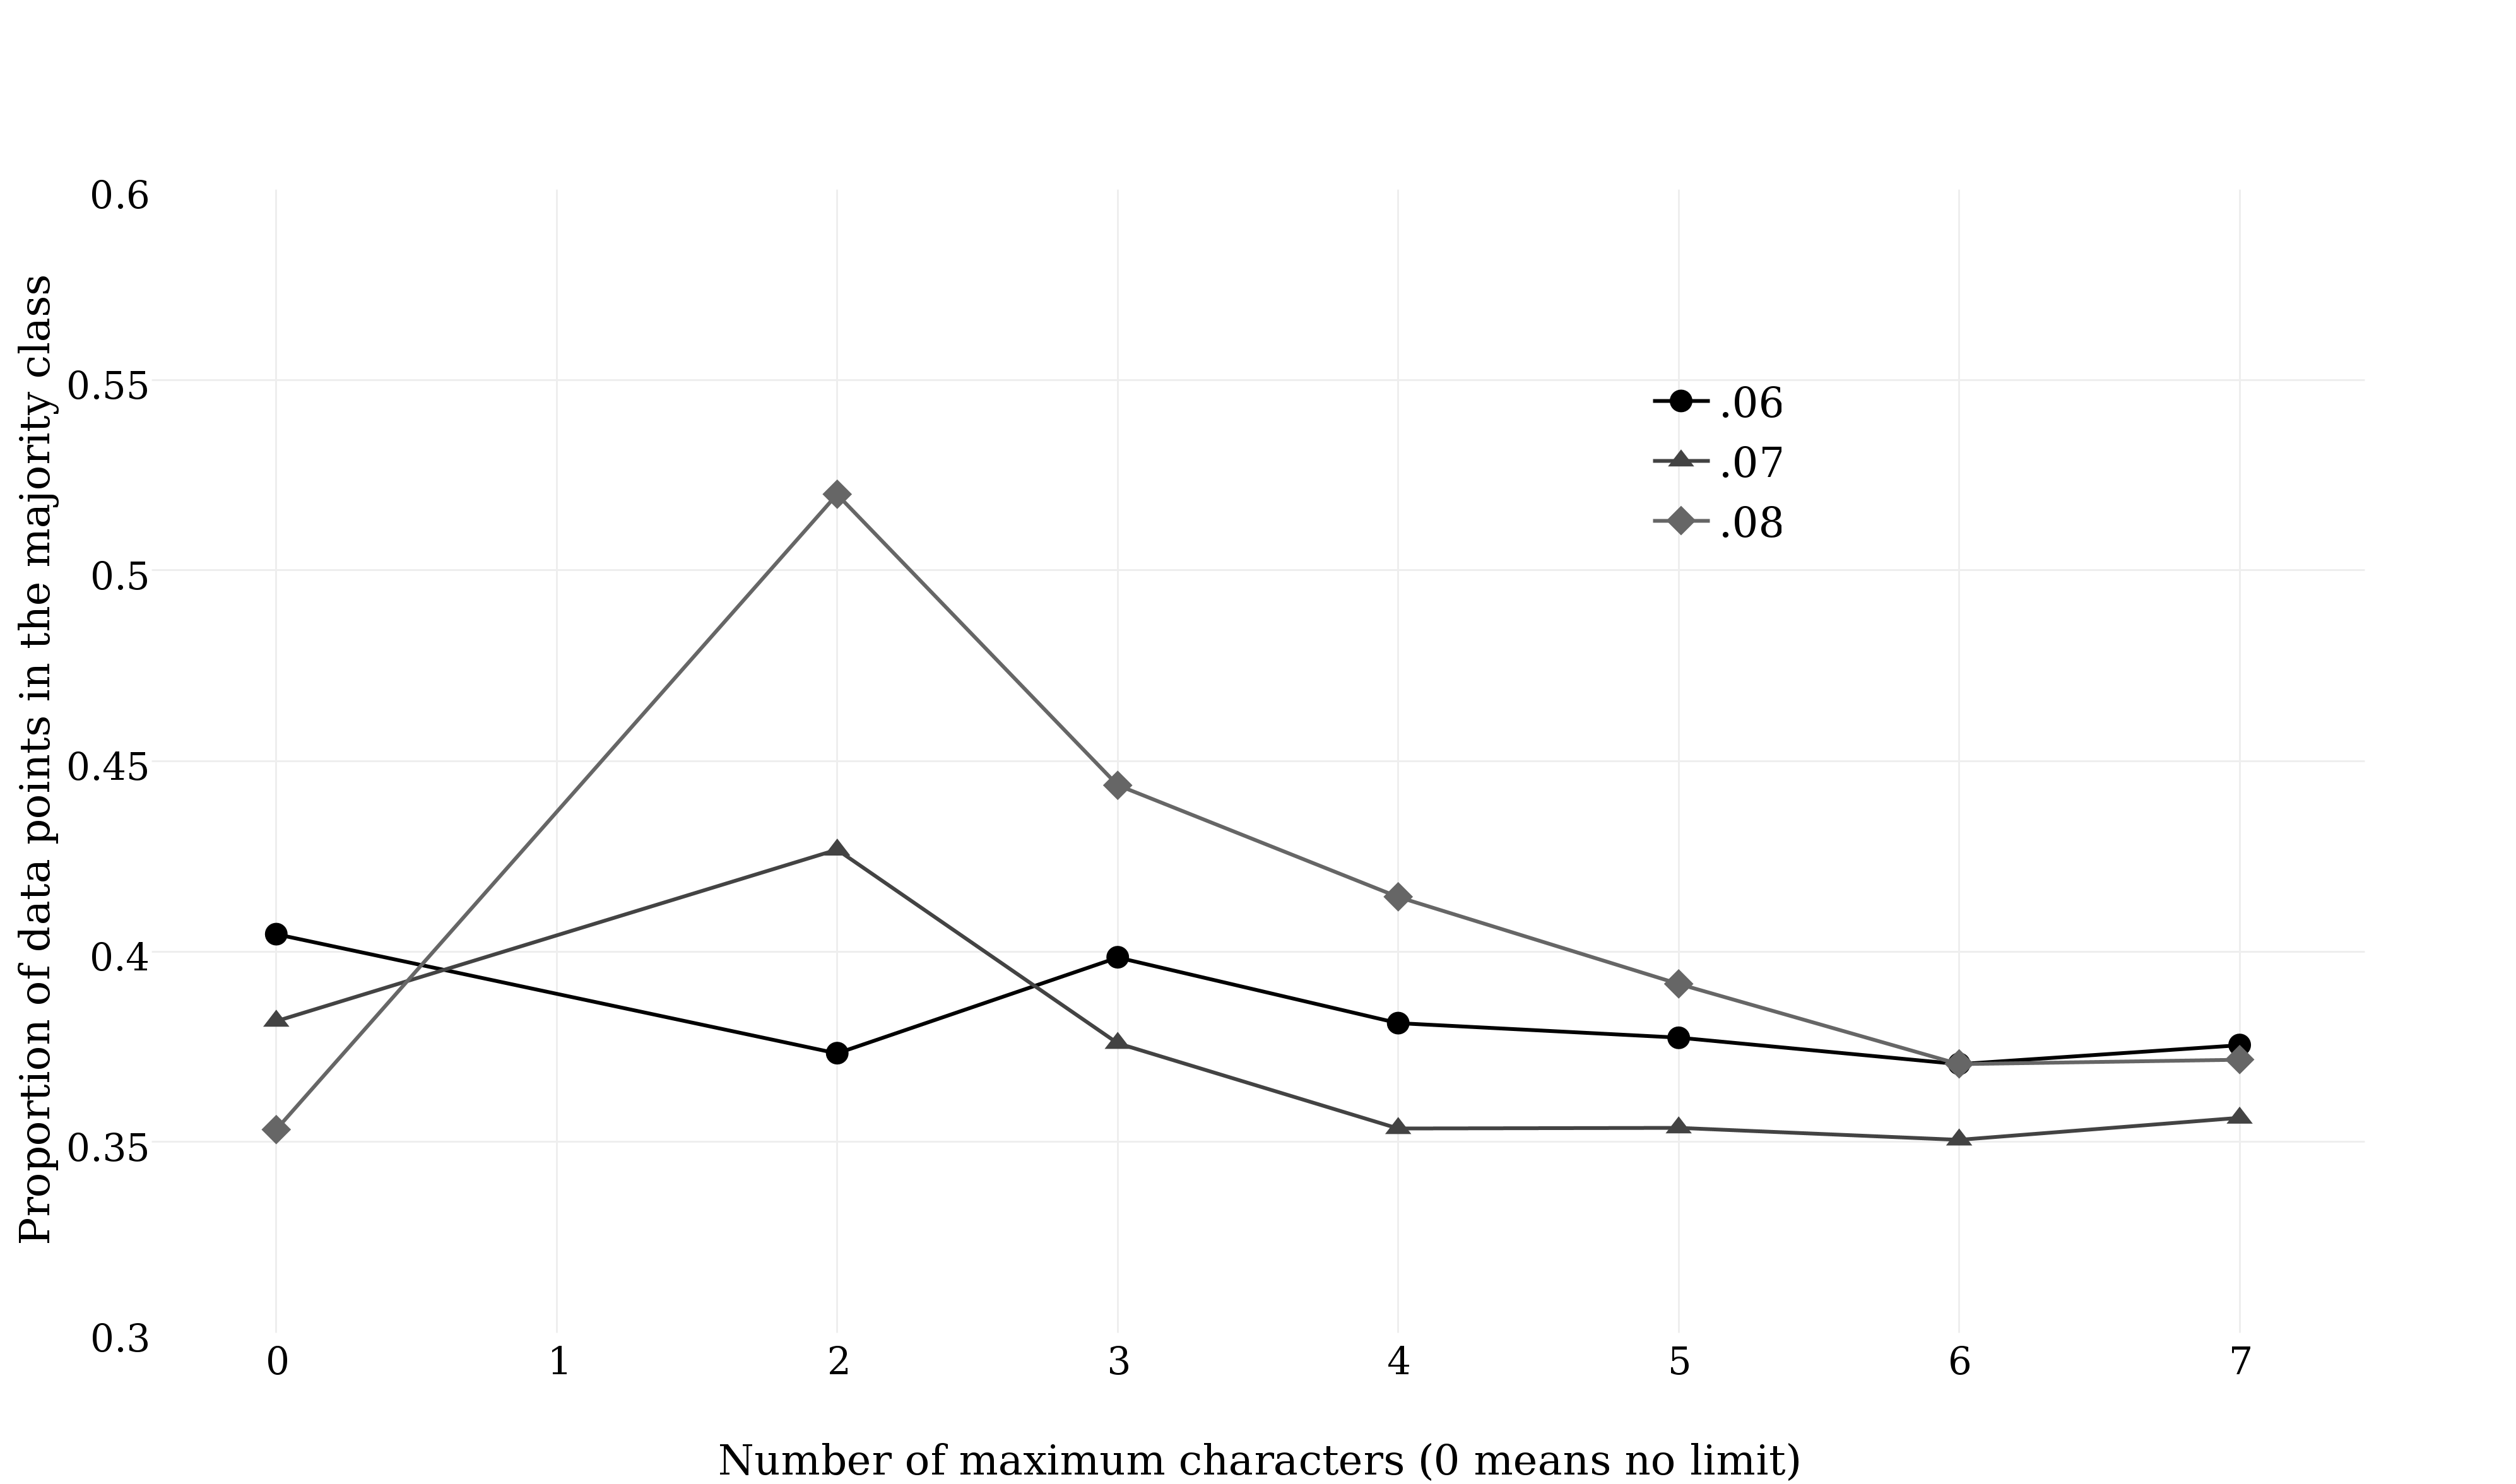
\includegraphics[scale=0.55]{figures/variation_alpha2}
	\caption{Proportion of data points in the majority class, over different values for the maximum number of characters ($N$), for 3 settings of the parameter $\alpha$.}
\label{fig:alpha}
\end{adjustwidth}
\end{figure}

In most (5 out of 7) cases, $\alpha=0.07$ makes the lowest number of points to be in the majority class. Either increasing or increasing $\alpha$ will generally increase this proportion. We will therefore use $0.07$ when labelling the data used to train the classifiers. Their performance is shown in Table~\ref{res:sent_variation}. The highest accuracy is again obtained using random forests and it is $0.867$. Note that although setting $\alpha$ to $0.06$ or $0.08$ will result in a drop in performance,  in both of those cases, the best accuracy still ranges between $0.75$ and $0.80$.

\begin{table}[h!]
\begin{adjustwidth}{-0.5in}{-0.5in}
\centering
\small
\begin{tabular}{ |c|c|c|c|c|c!{\vrule width 1.5pt}c|c| }
\cline{1-6}
\multicolumn{6}{ |c!{\vrule width 1.5pt} }{Configuration}\\
\hline
 & No. & Filter & Personas & Top topics & Edge & & \\
Classifier & nodes & personas & used & only & used & Baseline & \textbf{Accuracy} \\ \hline
\multirow{2}{*}{Decision tree} 
 & 2 & Yes & P, M & 1 & Yes & 0.427 & \textbf{0.600}\\
 & 2 & Yes & P, M & 1 & No & 0.427 & \textbf{0.667}\\ \hline
\multirow{2}{*}{Random forest} 
 & 2 & Yes & P & 7 & Yes & 0.427 & \textbf{0.800}\\
 & 2 & Yes & A, P, M & 6 & No & 0.427 & \textbf{0.867}\\ \hline
\multirow{2}{*}{SVM}
 & 2 & Yes & P & 4 & Yes & 0.427 & \textbf{0.733}\\
 & 2 & Yes & P & 4 & No &  0.427 & \textbf{0.733}\\ \hline
\end{tabular}
\caption{Best sentiment variation prediction accuracy, with $\alpha = 0.07$.}
\label{res:sent_variation}
\end{adjustwidth}
\end{table}

We have shown that predicting changes in inter-character sentiment is also feasible with our representation. Note that the baselines are notably smaller than in the previous task, since we sought to obtain roughly equally sized classes.

\subsubsection{Comparison of results between the 2 classification tasks}
When predicting changes in sentiment, for all 3 classifiers, the best accuracy is obtained when limiting the maximum number of nodes in a character graph ($N$) to 2. This is similar to the sentiment polarity classification task, in which the best results were obtained when using an $N \in \{2, 3\}$. We can offer a possible explanation for this bias in both of these cases. The sentiment trajectories of films will naturally include more events between the more central characters in the narrative, which can result in less erratic predictions, since the influence of outliers (e.g. from shortcoming in sentiment analysis) is limited.

Another common feature to note is the preference, in both tasks, to one of the 3 distributions in a character persona. While the choice of distributions varies for different classifiers, we can observe that in the sentiment polarity prediction task all the best-performing models were trained using (sometimes exclusively) the \textit{agent} distribution. This kind of preference is also observed in the sentiment variation task, but for the \textit{patient} distribution. We can speculate that such a bias seems to show that actions that the characters do themselves will better predict the overall sentiment of a relationship, while actions which the characters experience are more likely predictors of how relationships evolve in the timeline of the story.

One last thing to note is that for both tasks and for all classifiers, using the edge weight (i.e. number of scene co-occurrences of 2 characters) as an extra feature in the feature vectors either has no effect on or decreases classification accuracy. This would seem to indicate that the persona model is enough to predict inter-character sentiment. However, as earlier discussed, the best results were obtained for values of $N \le 3$, with nodes ranked by their degree centrality in the character graph. As a consequence, it is possible that using the edge weight only added noise to the data and the inter-character sentiment depends more on how central the characters are to the story than on an absolute measure of the frequency of their interactions. This claim can be supported by the fact that using the edge weight did not decrease accuracy when all the characters of a film were included (Table~\ref{res:full_set}).

\subsection{Predicting compound sentiment}
We have modelled previous tasks as classification problems. However, inter-character sentiment is a continuous numerical value, meaning we can also explore regression tasks. The broadest such task is simply predicting the value of inter-character compound sentiment. Attempting to obtain the best possible results, we will explore the whole space of configurations introduced in the sections above. Results are shown in Table~\ref{res:regression}. 

\begin{table}[ht!]
\begin{adjustwidth}{-0.5in}{-0.5in}
\centering
\small
\begin{tabular}{ |c|c|c|c|c|c!{\vrule width 1.5pt}c| }
\cline{1-6}
\multicolumn{6}{ |c!{\vrule width 1.5pt} }{Configuration}\\
\hline
 & No. & Filter & Personas & Top topics & Edge & \textbf{Mean squared}\\
Classifier & nodes & personas & used & only & used & \textbf{error} \\ \hline
\multirow{2}{*}{Linear regression} 
 & All & Yes & M & 7 & Yes & 10.19\\
 & All & Yes & M & 7 & No & 10.19\\ \hline
\multirow{2}{*}{Ridge regression} 
 & All & Yes & A, M & 7 & Yes & 10.30\\
 & All & Yes & A, M & 7 & No & 10.28\\ \hline
\multirow{2}{*}{\parbox{2.3cm}{Decision tree regression}}
 & All & Yes & A & 2 & Yes & 10.55\\
 & All & Yes & A & 2 & No & 10.50\\ \hline
\multirow{2}{*}{SVM regression}
 & All & Yes & A & 3 & Yes & 10.99\\
 & All & Yes & A & 3 & No & 10.99\\ \hline
\end{tabular}
\caption{Best sentiment polarity prediction accuracy.}
\label{res:regression}
\end{adjustwidth}
\end{table}


\chapter{Conclusions and future work}


\bibliographystyle{plain}
\bibliography{collection}

\appendix
%% Sample chapter file, for use in a thesis.
%% Don’t forget to put the \chapter{...} header onto each file.
\chapter{CMU Movie Summary Corpus preprocessing example}
\label{appendix:cmu}
This appendix supports the explanation is Section~\ref{sec:processing_cmu}. To illustrate the preprocessing steps that take the raw plot summaries and generate the input for the work described in \cite{Bamman2013} and used in this project, we will give a concrete example of a sentence in a plot summary, as it is passed through the preprocessing pipeline. For this we will use the first sentence in the Wikipedia plot summary for \textit{The Silence of the Lambs} (1994).

\begin{figure}[h!]
\centering
\begin{minipage}{14.5cm}
We start with the unprocessed sentence:
\vspace{1.5mm}
\begin{Verbatim}[frame=single]
Clarice Starling  is pulled from her training at the FBI Academy 
at Quantico, Virginia, by Jack Crawford  of the Bureau's Behavioral 
Science Unit.
\end{Verbatim}
\end{minipage}
\end{figure}

\begin{figure}[h!]
\centering
\begin{minipage}{14.5cm}
The sentence is tokenised, with tokens being split by spaces:
\vspace{1.5mm}
\begin{Verbatim}[frame=single]
Clarice Starling is pulled from her training at the FBI Academy at 
Quantico , Virginia , by Jack Crawford of the Bureau 's Behavioral 
Science Unit .
\end{Verbatim}
\end{minipage}
\end{figure}

\begin{figure}[h!]
\centering
\begin{minipage}{14.5cm}
Then, tokens are lemmatised (i.e. transformed into their canonical, non-inflected form):
\vspace{1.5mm}
\begin{Verbatim}[frame=single]
Clarice Starling be pull from she training at the FBI Academy at 
Quantico , Virginia , by Jack Crawford of the Bureau 's 
Behavioral Science Unit .
\end{Verbatim}
\end{minipage}
\end{figure}

\begin{figure}[h!]
\centering
\begin{minipage}{14.5cm}
The sentence is also annotated with part-of-speech (POS) tags:
\vspace{1.5mm}
\begin{Verbatim}[frame=single]
NNP NNP VBZ VBN IN PRP$ NN IN DT NNP NNP IN NNP , NNP , IN NNP 
NNP IN DT NNP POS NNP NNP NNP .	
\end{Verbatim}
\end{minipage}
\end{figure}

\begin{figure}[h!]
\centering
\begin{minipage}{14.5cm}
It is also annotated with the named entity information:
\vspace{1.5mm}
\begin{Verbatim}[frame=single]
PERSON PERSON O O O O O O O ORGANIZATION ORGANIZATION O 
LOCATION O LOCATION O O PERSON PERSON O O ORGANIZATION O 
ORGANIZATION ORGANIZATION ORGANIZATION O	
\end{Verbatim}
\end{minipage}
\end{figure}

\begin{figure}[h!]
\centering
\begin{minipage}{14.5cm}
Stanford typed dependencies are computed:
\vspace{1.5mm}
\begin{Verbatim}[frame=single]
[["nn",0,1],["nsubjpass",1,3],["auxpass",2,3],["poss",5,6],
["prep_from",6,3],["det",8,10],["nn",9,10],["prep_at",10,6],
["nn",12,14],["prep_at",14,3],["nn",17,18],["agent",18,3],
["det",20,21],["poss",21,25],["nn",23,25],["nn",24,25],
["prep_of",25,18]]	
\end{Verbatim}
\end{minipage}
\end{figure}

\begin{figure}[h!]
\centering
\begin{minipage}{14.5cm}
And the sentence is syntactically parsed:
\vspace{1.5mm}
\begin{Verbatim}[frame=single]
(ROOT (S (NP (NNP Clarice) (NNP Starling)) (VP (VBZ is) 
(VP (VBN pulled) (PP (IN from) (NP (NP (PRP$ her) (NN 
training)) (PP (IN at) (NP (DT the) (NNP FBI) (NNP Academy)))
)) (PP (IN at) (NP (NNP Quantico) (, ,) (NNP Virginia) (, ,)))
 (PP (IN by) (NP (NP (NNP Jack) (NNP Crawford)) (PP (IN of) 
 (NP (NP (DT the) (NNP Bureau) (POS 's)) (NNP Behavioral) (NNP 
 Science) (NNP Unit))))))) (. .)))
\end{Verbatim}
\end{minipage}
\end{figure}

\begin{figure}[h!]
\centering
\begin{minipage}{14.5cm}
Finally, each token is categorised as being an \textit{agent}, \textit{patient} or \textit{modifier} word based on its typed dependency (those which do not have one of the relevant dependencies are discarded). Coreference resolution is used to resolve the dependencies to the correct character. Where it is possible, character names are matched with Freebase entities, otherwise, an internal identifier is used. The final input file contains tuples of the form:
\vspace{1.5mm}
\begin{Verbatim}[frame=single]
/m/0k6g8c:t0.1.0:verb.contact:pull:a:agent
/m/0k6g8p:t2.2.0:verb.stative:lead:a:agent
/m/0k6g86:t3.0.0:verb.change:grow:a:nsubj
/m/0k6g86:t3.2.0:verb.communication:rebuff:a:nsubj
/m/0k6g86:t5.1.0:verb.communication:call:a:nsubj
/m/0k6g86:t5.2.0:verb.communication:tell:a:nsubj
/m/0k6g86:t8.0.0:verb.possession:offer:a:nsubj
/m/0k6g86:t8.4.0:verb.emotion:detest:a:nsubj
/m/03jrpdm:t9.0.0:verb.contact:kidnap:a:nsubj
/m/0k6g8c:t9.1.0:verb.communication:authorize:a:nsubj
/m/0k6g81:t9.2.0:verb.possession:offer:a:nsubj
/m/0k6g81:t9.4.0:verb.possession:provide:a:nsubj
/m/0k6g81:t10.2.0:verb.possession:give:a:nsubj
/m/0k6g8p:t11.0.0:verb.communication:record:a:nsubj
/m/0k6g8p:t11.1.0:verb.perception:reveal:a:nsubj
/m/0k6g86:t12.0.0:verb.communication:agree:a:nsubj
/m/0k6g86:t12.3.0:verb.perception:reveal:a:nsubj 
(...)
\end{Verbatim}
\end{minipage}
\end{figure}


\end{document}